\documentclass[a4paper]{article}
\usepackage{amsmath, amssymb, amsfonts}
\usepackage[margin=1in]{geometry}
\usepackage{graphicx}
\usepackage{tikz}
\usepackage{tikz-feynman}
\usepackage{esint}
\setlength{\parindent}{0em}
\setlength{\parskip}{1ex}

\DeclareFontFamily{U}{mathb}{}
\DeclareFontShape{U}{mathb}{m}{n}{<-> mathb10}{}
\DeclareSymbolFont{mathb}{U}{mathb}{m}{n}
\DeclareMathSymbol{\longrightsquigarrow}{1}{mathb}{"F9}

\newcommand{\vct}[1]{\overrightarrow{#1}}
\newcommand{\dif}{\mathrm{d}}
\newcommand{\pd}[2]{\frac{\partial {#1}}{\partial {#2}}}
\newcommand{\dd}[2]{\frac{\mathrm{d} {#1}}{\mathrm{d} {#2}}}
\newcommand{\C}{\mathbb{C}}
\newcommand{\R}{\mathbb{R}}
\newcommand{\Q}{\mathbb{Q}}
\newcommand{\Z}{\mathbb{Z}}
\newcommand{\N}{\mathbb{N}}
\newcommand{\fn}[3]{{#1}\colon {#2} \rightarrow {#3}}
\newcommand{\avg}[1]{\langle {#1} \rangle}
\newcommand{\Sum}[2][0]{\sum_{{#2} = {#1}}^{\infty}}
\newcommand{\Lim}[1]{\lim_{{#1} \rightarrow \infty}}
\newcommand{\Binom}[2]{\begin{pmatrix} {#1} \cr {#2} \end{pmatrix}}
\newcommand{\duline}[1]{\underline{\underline{#1}}}
\newcommand{\anti}[1]{\overline{#1}}

\begin{document}
\paragraph{Feynmanovi diagrami.} Reakcijo ponazorimo s sledečimi predpisi:
\begin{align*}
    \longrightsquigarrow: & \hspace{1cm}\text{Virtualni foton oz. nosilec interakcije} \\
    \longrightarrow: & \hspace{1cm}\text{Delec} \\
    \longleftarrow: & \hspace{1cm}\text{Antidelec} \\
\end{align*}
V splošnem nepolne črte predstavljajo nosilce interakcij: fotone (EM  interakcija), gluone (močna interakcija) in \(W^\pm,Z\) bozone (šibka interakcija).
Z \(\alpha\) označimo sklopitveno konstanto interakcije, ki jo potrebujemo za amplitudo prehoda. Propagator interakcije izračunamo po formuli \[\frac{1}{q^2 + M^2c^4}\]
\(M\) je masa nosilca interakcije.
\paragraph{Šibka interakcija.} Za primer vzemimo razpad $\beta$: $n \to p e^- \,\overline{\nu}_e$ \\
Pri opisani reakciji je nosilec šibke interakcije bozon \(W^-\) z energijo \(M_{W}c^2 = 95\,\mathrm{GeV}\). Sklopitveno konstanto tokrat označimo
z \(\alpha_W\). \\[3mm]
Potek reakcije: Eden od kvarkov \(d\) odda virtualni \(W^-\) in se pri tem spremeni v kvark \(u\). Bozon 'razpade' v elektron \(e^-\) in elektronski antinevtrino \(\overline{\nu}_e\).
% Narišimo primer Feynmanovega diagrama za to interakcijo:
%\begin{tikzpicture}
%    \begin{feynman}
%        \feynmandiagram [horizontal=u1in to u1out] {
%            u1in [particle=\(u\)] -- [fermion] -- u1out [particle=\(u\)];
%            d1in [particle=\(u\)] -- [fermion] -- d1out [particle=\(u\)];
%            d2in [particle=\(u\)] -- [fermion] x -- [fermion] -- u2out [particle=\(u\)];
%            x -- [boson=\(W^-\)] -- y;
%            y -- [fermion] -- el [particle=\(e^-\)]
%            y -- [fermion] -- nev [particle=\(\overline{\nu}_e\)]
%        };
%    \end{feynman}
%\end{tikzpicture}
$$\mathcal{M} \propto \sqrt{\alpha_w}\frac{1}{(p-p')^2 - M_w^2c^4}\sqrt{\alpha_w} = \frac{\alpha_w}{q^2-M_w^2c^4}$$
$$|\mathcal{M}|^2 \propto \alpha^2 \left(\frac{\alpha_w}{q^2-M_w^2c^4}\right)^2 \sim \frac{\alpha_w^2}{M_w^4c^8}$$
Drugi primeri: \\
\begin{itemize}
    \item \(D^0 \to K^-e^+\nu_e\): Kvark \(c\) odda virtualni \(W^+\) bozon in se spremeni v kvark \(s\). Iz bozona nastaneta \(e^+\) in \(\nu_e\).
    \item \(\pi^+ \to \mu^+\nu_\mu\): Tu oba kvarka (\(u\) in \(\overline{d}\)) izgineta in oddata bozon \(W^+\). Iz tega nastaneta \(\mu^+\) in \(\nu_\mu\).
    \item \(D^0 \to K^-\pi^+\): Kvark \(c\) odda bozon in se spremeni v kvark \(s\). Iz bozona nastaneta kvarka \(u\anti{d}\), ki skupaj tvorita \(\pi^+\).
    \item \(D^0 \to K^-\pi^+\): Kvark \(c\) odda bozon in se spremeni v kvark \(d\). Iz bozona nastaneta kvarka \(u\anti{d}\), ki skupaj tvorita \(\pi^+\).
\end{itemize}
\paragraph{Prehodi med kvarki.} Narišemo tabelo prehodov med kvarki.
\begin{figure}[h!]
    \centering
    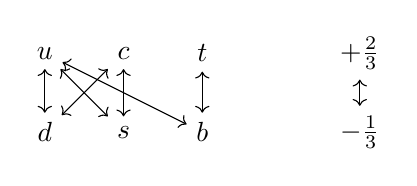
\begin{tikzpicture}
        \node (u) at (-1, 0.5) {\(u\)};
        \node (d) at (-1, -0.5) {\(d\)};
        \node (c) at (0, 0.5) {\(c\)};
        \node (s) at (0, -0.5) {\(s\)};
        \node (t) at (1, 0.5) {\(t\)};
        \node (b) at (1, -0.5) {\(b\)};

        \node (+) at (3, 0.5) {\(+\frac{2}{3}\)};
        \node (-) at (3, -0.5) {\(-\frac{1}{3}\)};

        \draw[<->] (u) -- (d);
        \draw[<->] (u) -- (s);
        \draw[<->] (u) -- (b);
        \draw[<->] (c) -- (d);
        \draw[<->] (c) -- (s);
        \draw[<->] (t) -- (b);
        \draw[<->] (+) -- (-);
    \end{tikzpicture}
\end{figure}
\paragraph{Verjetnosti za prehode.} Imamo matriko Cabibbo-Kobayashi-Maskawa, ki opisuje potenciale med kvarki. Je unitarna, kompleksna matrika.
$$V_{CKM} = \begin{matrix}
    & \begin{matrix} 
    d & s & b
    \end{matrix} \\
    \begin{matrix}
        u \\ c \\ t
    \end{matrix} &
    \begin{bmatrix}
        V_{ud} & V_{us} & V_{ub} \\
        V_{cd} & V_{cs} & V_{cb} \\
        V_{td} & V_{ts} & V_{tb}
    \end{bmatrix} \\
    & \\
\end{matrix}$$
Wolfsteinova parametrizacija:
$$V_{CKM} = \begin{bmatrix}
    1 - \lambda^2/2 & \lambda & A\lambda^3(\rho + i\eta) \\
    -\lambda & 1 - \lambda^2/2 & A\lambda^2 \\
    A\lambda^3(1 - \rho - i\eta) & A \lambda^2 & 1
\end{bmatrix}$$
Po Wolfsteinovi parametrizaciji je
\begin{itemize}
    \item $\lambda = 0.225$
    \item $A = 0.826$
    \item $\eta = 0.348$
    \item $\rho = 0.159$
\end{itemize}
Tedaj dobimo matriko absolutnih vrednosti
$$V = \begin{bmatrix}
    0.974 & 0.225 & 0.004 \\
    0.225 & 0.974 & 0.041 \\
    0.009 & 0.041 & 0.999 \\
\end{bmatrix}$$
Pri šibki interakciji se en kvark spremeni v drugega, nastanejo novi kvarki in tako naprej. Amplitudo ($\mathcal{M}$) dobimo iz matričnega elementa, na primer:
$$D^0 \to K^- \pi^+$$
Pri reakciji se $\anti{u}$ ohrani, $c$ postane $s$, nastaneta pa $u$ in $\anti{d}$. Amplituda je tedaj enaka
$$\mathcal{M} \propto \sqrt{\alpha_w}\sqrt{\alpha_w}V_{cs}V_{ud}$$
\paragraph{Pretvorba delec-antidelec.} Primer: $$K^0 \to \anti{K^0}$$
$$\widehat{H}\psi = \widehat{E}\psi$$
reakcija poteka z neko časovno odvisnostjo: $$|K^0\rangle \to a(t) |K^0\rangle + b(t)|\anti{K^0}\rangle$$
Ker se tako $|K^0\rangle$ kot $|\anti{K^0}\rangle$ spreminjata skozi čas, nobena od njiju ne mora biti lastna vrednost, lahko pa je njuna linearna kombinacija:
$$|K_1\rangle = \cos\vartheta |K^0\rangle + \sin\vartheta |\anti{K^0}\rangle$$
$$|K_2\rangle = -\sin\vartheta |K^0\rangle + \cos\vartheta |\anti{K^0}\rangle$$
Iz razlogov, v katere se zaenkrat ne bomo poglabljali, je $\vartheta = 45^\circ$. Dobili smo lastni stanji $\widehat{H}$.
$$\widehat{H} |K_1\rangle = E_1 |K_1\rangle$$
$$\widehat{H} |K_2\rangle = E_2 |K_2\rangle$$
$$|K_1(t)\rangle = |K_1(t=0)\rangle e^{-\frac{iE_1t}{\hbar}}$$
$$|K_2(t)\rangle = |K_2(t=0)\rangle e^{-\frac{iE_2t}{\hbar}}$$
Vrh tega lahko zapišemo $|K_1\rangle - |K_1\rangle = \sqrt{2}|K_0\rangle$ in na podlagi tega izrazimo $|K^0\rangle$ in $|\anti{K^0}\rangle$. S tem dobimo valovno funkcijo
$$|\psi\rangle = |K^0\rangle = \frac{1}{\sqrt{2}} \left(|K_1(0)\rangle e^{-\frac{iE_1t}{\hbar}} - |K_2(0)\rangle e^{-\frac{iE_2t}{\hbar}}\right)$$
Če želimo izraziti verjetnost, da se bo $K^0$ pretvoril v $\anti{K^0}$, moramo izračunati skalarni produkt:
$$\avg{\anti{K^0}|\psi(t)} = \left(\frac{1}{\sqrt{2}}\langle K_1|+ \langle K_2|\right)\left(\frac{1}{\sqrt{2}}\|K_1\rangle e^{-\frac{iE_1t}{\hbar}} - |K_2\rangle e^{-\frac{iE_2t}{\hbar}}\right)$$
$$= \frac{1}{2}\left(e^{-\frac{iE_1 t}{\hbar}} - e^{-\frac{iE_2t}{\hbar}}\right)$$
\end{document}